\chapter{基于强化学习的行人控制}

\section{环境配置}

本研究主要目标是用强化学习算法(PPO、PID、DQN)训练优化行人控制系统,核心是评估这些算法在复杂动态环境里的性能表现。为此,所有深度学习训练与实验都在功能强大的 Carla 仿真平台开展。Carla 平台有多样城市环境,涵盖各类道路、建筑风格、车辆模型、行人行为,能模拟真实城市交通复杂性,这让它成为自动驾驶研究和智能体训练的理想测试平台。​

\begin{figure}[H]
    \centering
    \includegraphics[width=1\textwidth]{images/town1.pdf}
    \caption{Carla中的Town1俯视图}
    \label{fig:town1}
\end{figure}

Carla 是专为自动驾驶研究设计的开源模拟平台,支持相机、激光雷达(LiDAR)、惯性测量单元(IMU)等多种传感器集成,能模拟含道路、交通信号灯、行人及其他交通参与者的复杂城市环境,为强化学习、路径规划、感知与控制算法开发提供高度可定制虚拟环境。本研究借 Carla 的 Python API 与仿真环境交互,实现行人运动控制并收集环境数据用于学习,该 API 能以编程模拟行人、车辆、交通灯等动态因素,还能实时获取各类传感器数据,给算法训练测试提供丰富信息。​

本研究因训练测试需求及研究者个人电脑计算能力限制选择 Carla 仿真平台 Town01 地图作为实验环境。Town01 作为 Carla 平台标准城市地图之一如图 \ref {fig:town1} 所示,包含多种城市道路结构、交通标志、建筑物、行人及交通工具等元素,设计旨在模拟真实城市交通环境并提供丰富具代表性的测试场景。该地图具备较高城市仿真还原度,结构涵盖多个复杂布局的城市道路与交叉口以重构现实交通网络与流动模式,集成私家车、公务车、公交车等多类型交通工具及行人对象、交通信号灯系统模拟典型城市运行状态,强化学习训练中除道路建筑等静态构造物外,还引入移动车辆与行人个体等具行为逻辑的动态障碍物以提升路径规划与避障策略的难度与真实性。

\section{PID(Proportional-Integral-Derivative)控制算法}

\begin{algorithm}[H]
	\caption{自适应PID控制算法}
	\begin{algorithmic}[1]
	\STATE 初始化参数$K_p^0$, $K_i^0$, $K_d^0$  % 改为 \STATE
	\WHILE{系统运行}
 	\STATE 获取激光雷达数据$L_t$
  	\STATE 计算障碍物距离$d_{obs} = \min(L_t)$
  	\IF{$d_{obs} < 5m$}
    	\STATE $K_p \gets 1.2K_p^0$
    	\STATE $K_d \gets 1.5K_d^0$
  	\ENDIF
  	\STATE 执行PID计算
	\ENDWHILE
	\end{algorithmic}
\end{algorithm}

\subsection{PID控制算法建模}

\subsubsection{控制方程推导}
离散PID控制算法表示为:
\begin{equation}
	u(k) = K_p e(k) + K_i T \sum_{i=0}^k e(i) + K_d \frac{e(k)-e(k-1)}{T}
\end{equation}
其中,$T=0.005s$为采样周期,$e(k)$为第$k$时刻的横向偏差。

\subsubsection{参数整定策略}
通过Ziegler-Nichols临界比例法确定基础参数后,结合实际场景进行优化:
转向控制参数:$K_p=0.8$, $K_i=0.001$, $K_d=0.2$\\
速度控制参数:$K_p=0.5$, $K_i=0.01$, $K_d=0.1$

\subsubsection{PID控制原理}

PID控制算法通过比例(P)、积分(I)与微分(D)三项协同工作实现对目标系统的控制,其数学表达如下:
\[
u(t) = K_p e(t) + K_i \int_0^t e(\tau) d\tau + K_d \frac{d}{dt} e(t)
\]
 $e(t)$ 表示当前时刻控制误差而 $u(t)$ 为控制器输出量,该控制器由三部分构成:

比例项 $K_p e(t)$ 通过调节比例系数 $K_p$ 对当前误差快速响应以修正偏离目标行为并增强响应速度和控制强度,积分项 $K_i \int_0^t e(\tau) d\tau$  通过累计过去误差补偿长时间累积的稳态偏差以提高系统长期控制精度,微分项  $K_d \frac{d}{dt} e(t)$ 根据误差变化速率预测调整以抑制系统振荡并提升稳定性与鲁棒性。

三者协同可在多种工程系统中实现较优的动态性能与稳态性能平衡,广泛应用于温度调节、伺服控制、轨迹跟踪等自动化控制场景。

\subsection{算法实现与效果可视化}

\subsubsection{传感器数据处理}

激光雷达传感器提供了高精度的三维点云信息,系统通过一套完整的预处理与分析流程将其转换为可用于导航决策的结构化信息。数据处理流程主要包括以下几个环节:

首先,系统对原始点云数据进行初步筛选,设定感知范围为半径不超过8米、水平视角位于前向60°范围内的空间区域,滤除无效测点与边缘噪声数据,从而减少冗余信息并提升处理效率。其次,在障碍物识别阶段,引入基于密度的空间聚类算法(改进版DBSCAN),设定聚类半径阈值 $\epsilon=0.5m$ 与最小邻居点数 $MinPts=5$,实现对局部高密度点云区域的有效分离,进而标定出潜在障碍物目标。最后,系统对已识别障碍物执行威胁评估,通过计算最短距离 $d_{min}$ 以及相对速度 $v_{rel}$ 等关键指标,辅助行为决策模块判断是否采取避障策略或调整路径规划。

该处理流程在保证实时性的基础上,提升了环境建模的准确性,为下游控制算法提供了可靠支持。

\subsubsection{动态权重融合算法}
目标向量$\vec{T}$与避障向量$\vec{A}$的融合策略:
\begin{equation}
	\vec{C} = \alpha \vec{T} + (1-\alpha)\vec{A}
\end{equation}
其中权重系数$\alpha$的动态调整规则为:
\begin{equation}
    \alpha = 
    \begin{cases}
        0.05, & d_{\text{min}} \leq 1\ \text{m} \\
        0.8(1 - e^{-0.5d_{\text{min}}}), & 1\ \text{m} < d_{\text{min}} \leq 5\ \text{m} \\
        1, & d_{\text{min}} > 5\ \text{m}
    \end{cases}
\end{equation}

\subsubsection{核心模块功能解析}

系统核心功能模块由若干关键类构成,分别负责路径控制、传感器数据处理、误差计算与控制环执行等任务,具体实现如下:

PIDController类承担基本的控制策略计算职责,其中\texttt{compute()}函数实现了具备抗积分饱和能力的PID控制逻辑,在保证控制稳定性的同时避免积分项过大造成系统震荡;\texttt{reset()}函数用于在检测到碰撞事件后清空累计误差,确保恢复控制时状态重置合理,有助于系统稳定恢复。

PIDPedestrianEnv类集成了环境感知与路径控制的多项功能。在感知方面,\texttt{\_process\_lidar()}函数对激光雷达点云数据进行实时处理,限定分析区域为前向60度扇形,最大探测距离为8米,随后采用DBSCAN聚类算法($\epsilon=0.5$ m)识别局部障碍物簇,实现高效环境建模。在路径误差估计方面,\texttt{calculate\_errors()}函数将目标方向与避障方向融合为一个期望方向向量,并根据当前任务阶段动态调整加权系数(取值范围为$[0.05, 0.95]$),再将该向量投影至局部坐标系以计算横向与纵向偏差,为后续控制指令提供误差信息支持。

控制执行层 \texttt{run\_control\_loop()}函数以 200Hz 高频运行保证控制精度与响应速度,速度控制通过引入非线性安全函数$v_{\text{safe}} = (\frac{d}{5})^{1.5} \cdot 3.0$动态调节移动速度确保接近障碍物时具备充分制动空间,系统在碰撞时自动触发后退 1 米后随机旋转 90 度重新导航的恢复策略提升鲁棒性与自主回复能力,该模块紧密集成感知规划与控制环节在确保实时性的同时有效提升导航稳定性与安全性。

\subsubsection{传感器系统架构}
\begin{figure}[H]
    \centering
    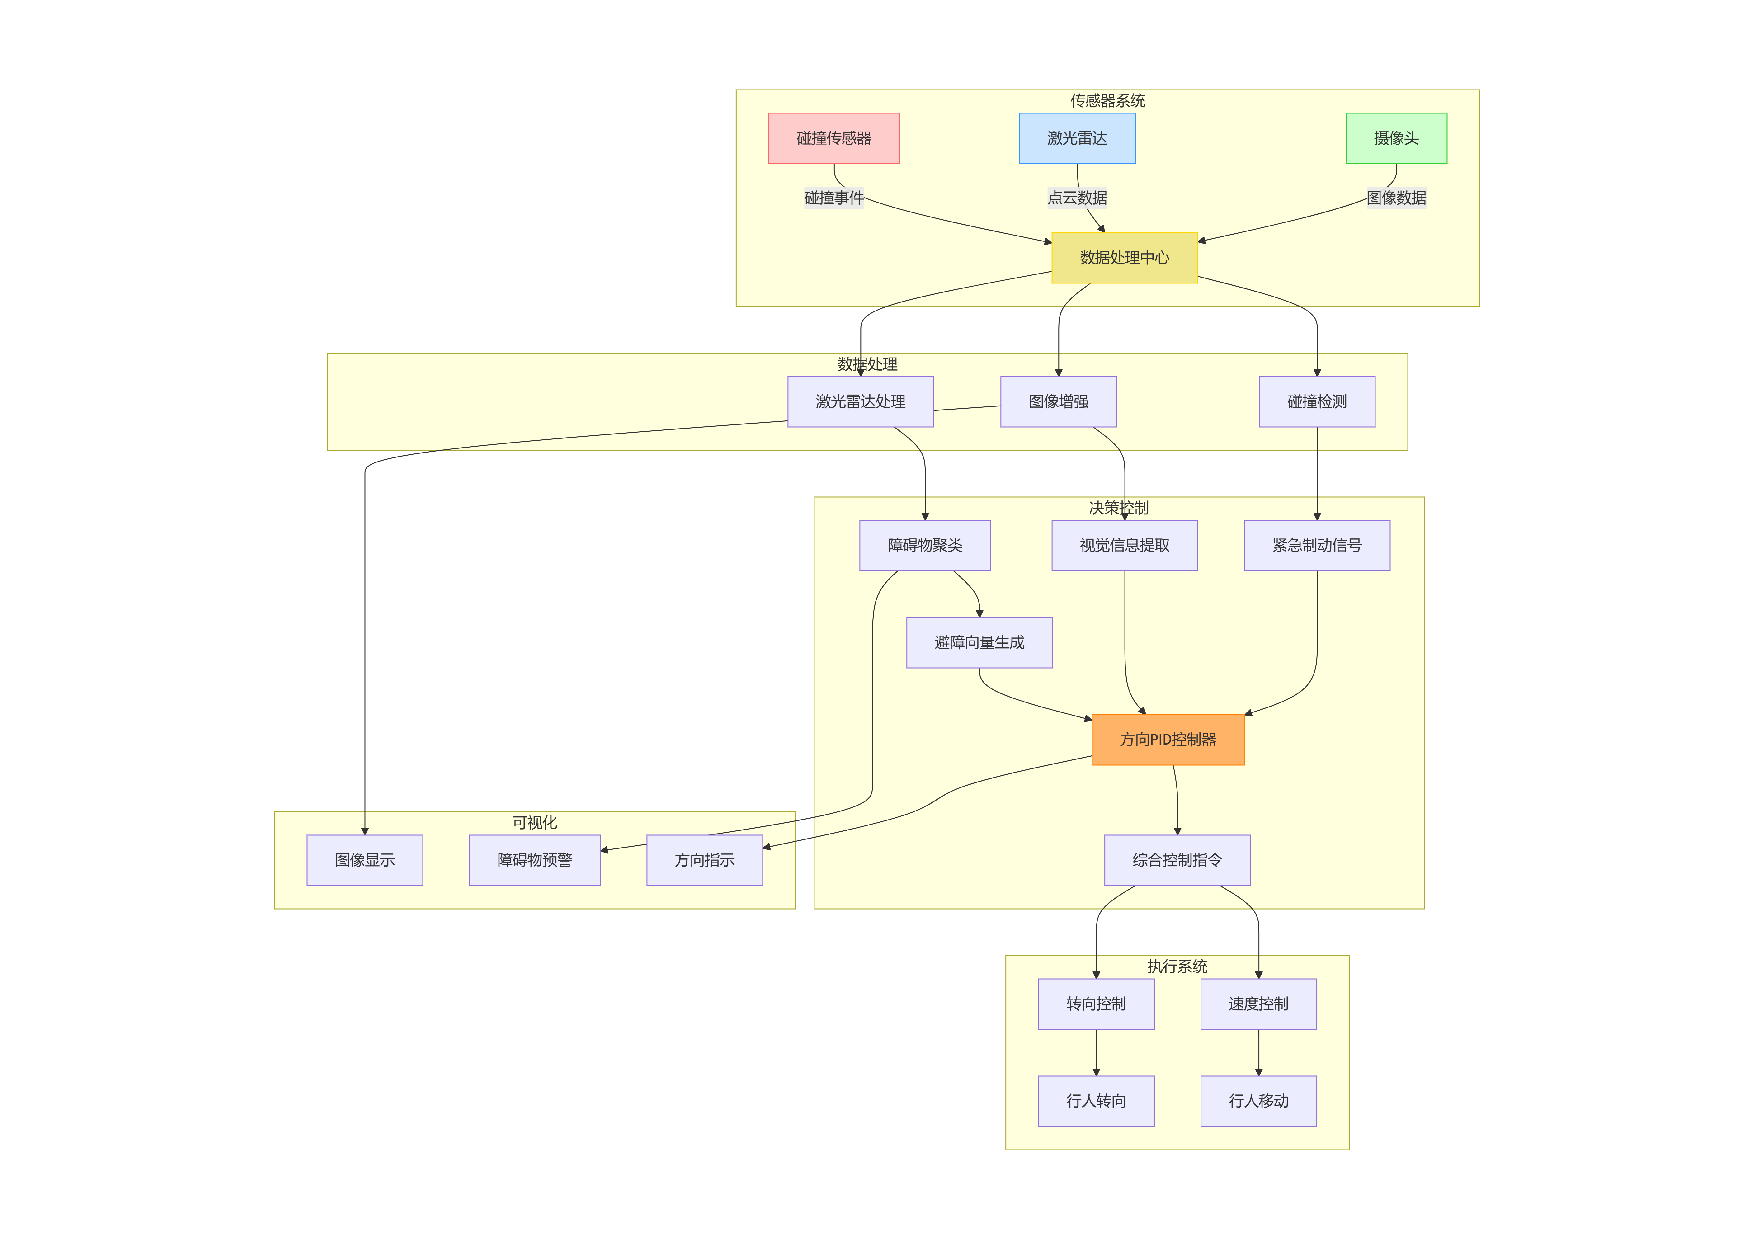
\includegraphics[width=1\textwidth]{images/sensor_architecture.pdf}
    \caption{多传感器数据融合架构}
    \label{fig:sensor}
\end{figure}

\subsection{实验结果分析}

为评估系统导航控制实际性能本节从避障效果、路径偏差控制与系统响应行为等维度分析实验结果并基于观察提出优化方向。系统在 100 次独立实验中避障成功 94 次成功率达93.7\% 表明控制策略在典型场景下具备较强鲁棒性与稳定性,实际行进路径相较理论路径平均偏差  $0.45 \pm 0.12$ 米显示动态环境中轨迹一致性较好,特定紧急避障情境中因障碍物突现或多障碍干扰出现最大18.7\%瞬时过冲。

图~\ref{fig:pid_obstacle} 展示智能体面对广告牌类障碍物时的避障行为,绿色箭头为导航目标方向、红色箭头为避障方向(仅障碍检测后可见)、蓝色箭头为实际前进方向,图像生成后经锐化及亮度对比度优化提升细节与视觉清晰度便于观察导航方向向量变化。

\begin{figure}[H]
    \centering
    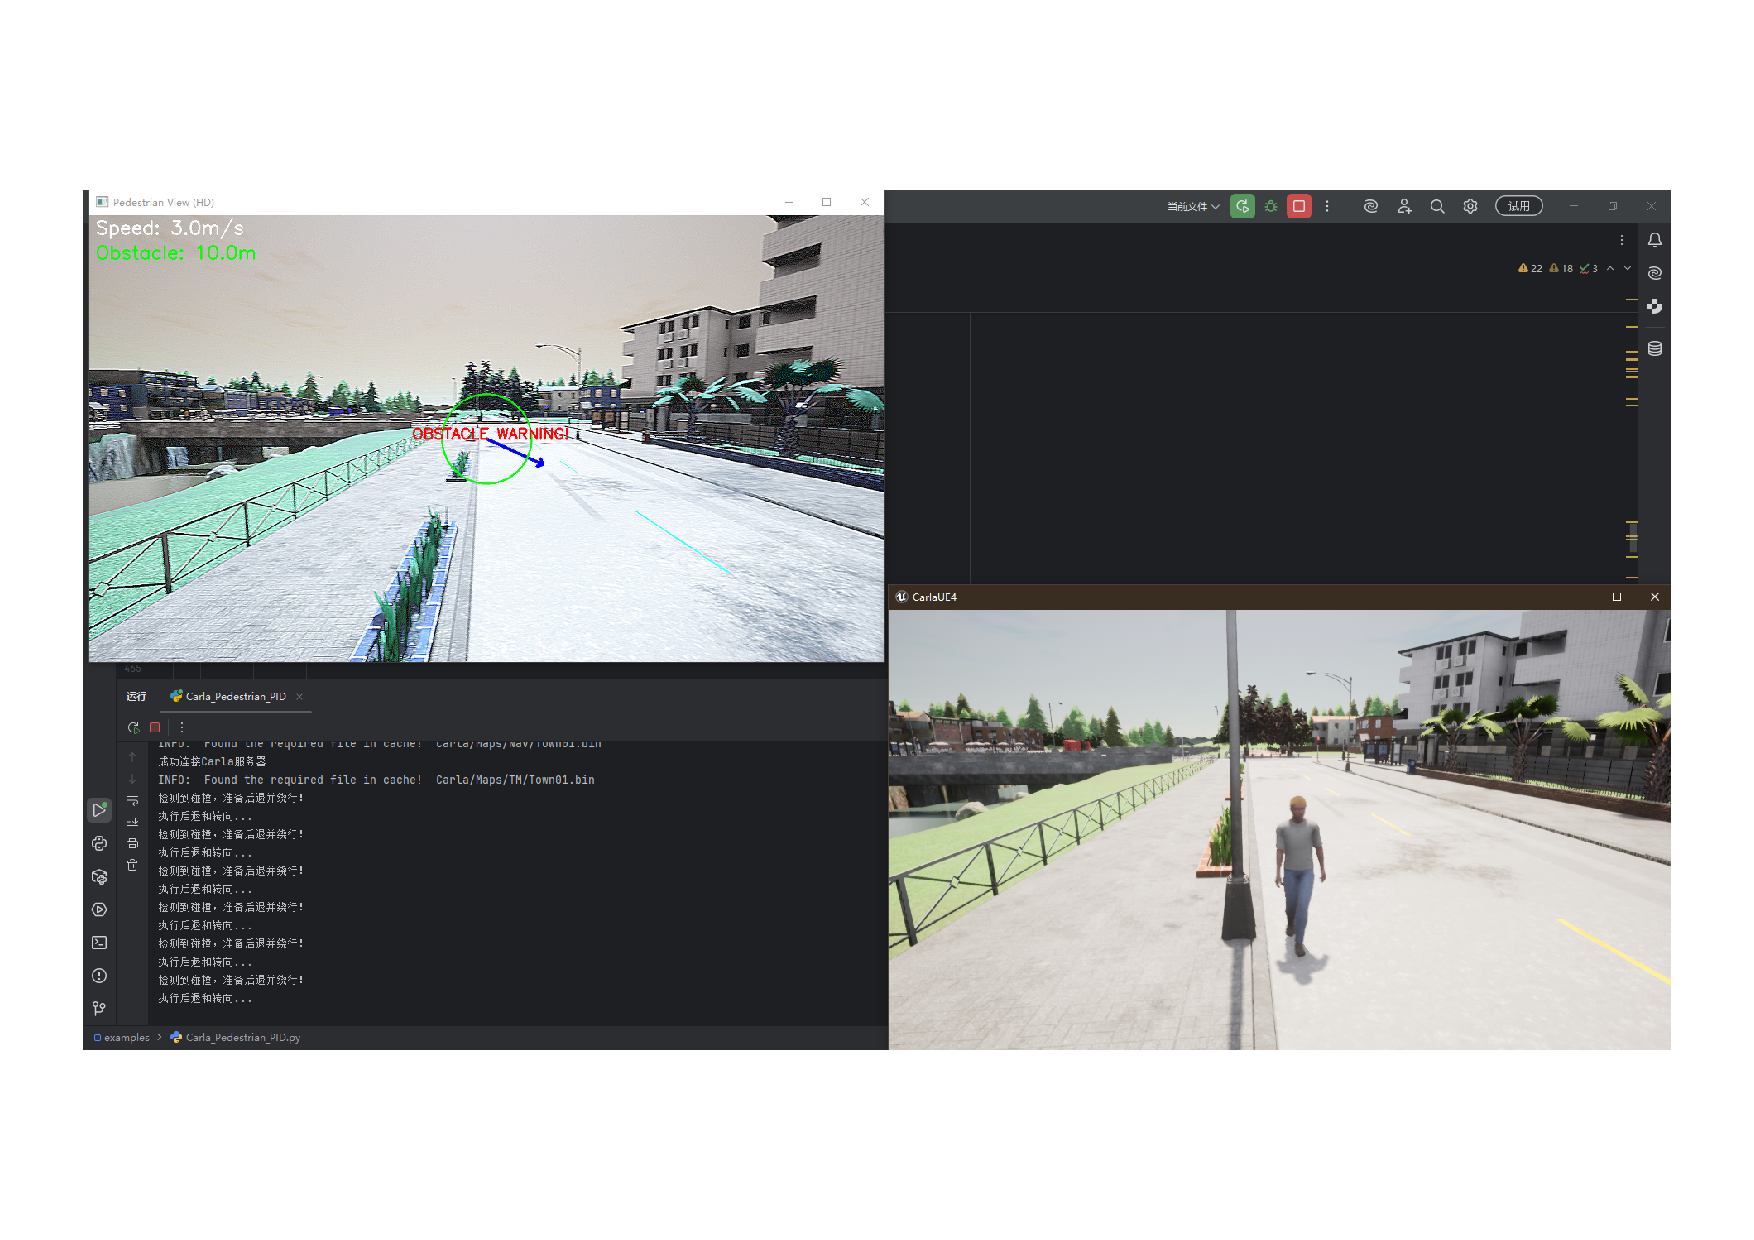
\includegraphics[width=1\textwidth]{images/obstacle_avoidance.pdf}
    \caption{行人智能体通过PID控制进行避障的示意图}
    \label{fig:pid_obstacle}
\end{figure}

基于实验表现系统功能实现已具良好基础但仍有提升空间,优化方向主要包括引入自适应 PID 参数调节机制提升不同场景响应灵活性、融合视觉语义信息提升障碍物识别分类精度与避障决策语境感知能力、采用模型预测控制(Model Predictive Control, MPC)方法优化路径平滑性与前瞻性减少复杂场景路径震荡问题。

\section{DQN(Deep Q-Network)算法}

\begin{algorithm}[H]
    \caption{DQN训练算法}
    \begin{algorithmic}[1]
    \STATE 初始化环境与模型
    \STATE 设置动作空间与状态空间
    \WHILE{训练过程中}
        \STATE 进行环境重置,获取初始观测$O_0$
        \FOR{每个训练步骤}
            \STATE 根据当前策略选择动作$a_t$
            \STATE 执行动作$a_t$,获得新的观测$O_{t+1}$,奖励$R_t$
            \STATE 存储经验$(O_t, a_t, R_t, O_{t+1})$
            \STATE 从经验池中采样批量数据进行更新
            \STATE 使用DQN算法更新Q网络
        \ENDFOR
    \ENDWHILE
    \end{algorithmic}
\end{algorithm}

\subsection{Q-learning公式}

在引入目标网络机制后,Q-learning算法的更新策略得到进一步优化,其Q值更新公式表达如下:
\[
Q(s_t,a_t) \leftarrow Q(s_t,a_t) + \alpha\left[r_t + \gamma \max_{a'}Q_{\text{target}}(s_{t+1},a') - Q(s_t,a_t)\right]
\]
该公式表示智能体在状态 $s_t$ 采取动作 $a_t$ 后,根据获得的即时奖励 $r_t$ 和下一状态 $s_{t+1}$ 的最大期望收益,调整当前状态-动作对的估值。其中各参数的含义如下:

学习率 $\alpha=10^{-4}$ 控制Q值更新的幅度,数值越小则代表对新信息的更新越缓慢(对应代码中的 \texttt{learning\_rate=1e-4});折扣因子 $\gamma=0.99$ 用于衡量未来回报的重要性,较高的折扣因子表明模型更注重长期收益(对应代码中的 \texttt{gamma=0.99})。此外,$Q_{\text{target}}$ 表示由目标网络计算得到的下一状态的最大Q值,用于提升估值过程的稳定性,避免在策略训练初期因频繁更新而导致震荡。

该更新机制能够在保留传统Q-learning策略探索性的基础上,通过固定目标网络参数进行延迟更新,有效缓解训练不稳定的问题,特别适用于深度强化学习中的高维状态空间建模场景。

\subsection{双网络架构设计}

为提升训练稳定性与估值精度,系统采用双网络架构,由在线网络(Online Network)与目标网络(Target Network)组成,分别承担策略更新与价值估计的不同功能。

在线网络用于实时学习当前策略,其结构为两层全连接神经网络,每层节点数为256,采用ReLU作为激活函数(对应代码设置为 \texttt{activation\_fn=torch.nn.ReLU}),在每一步梯度下降中更新权重参数 $\theta_{\text{online}}$,确保模型对最新状态反馈做出及时响应。

目标网络结构与在线网络保持一致,但其参数更新方式采用“硬更新”机制,即以固定步数间隔将在线网络的权重直接复制至目标网络。该同步过程公式如下所示:
\[
\theta_{\text{target}} \leftarrow \theta_{\text{online}}
\]
在具体实现中,目标网络每1000步执行一次参数同步(对应代码参数为 \texttt{target\_upda\\te\_interval=1000}),通过延迟更新策略降低了目标Q值波动,增强了训练过程的收敛性。

\subsection{经验回放机制}

经验回放(Experience Replay)机制用于缓解样本相关性对训练收敛的负面影响,系统通过构建经验池与延迟学习机制提升数据利用率与策略泛化能力。

经验池用于存储智能体在交互过程中收集的状态-动作-奖励-下一状态四元组,容量设置为 $10^5$ 条经验(对应代码参数为 \texttt{buffer\_size=100000}),每次训练从中均匀随机采样形成小批量数据,批次大小设为128条样本(\texttt{batch\_size=128}),以提升训练的稳定性与样本多样性。

在模型训练初期,系统采用延迟学习策略,即前1000步不进行参数更新,仅用于填充经验池(设置为 \texttt{learning\_starts=1000}),之后每隔4步执行一次策略网络的权重更新,从而保证网络初始训练基于足够多样的经验。

探索行为采用$\epsilon$-greedy策略控制动作选择过程,在训练初期以较高概率随机探索,随着训练步数增加逐步降低随机性。初始探索率 $\epsilon=1.0$,线性衰减至 $\epsilon=0.05$,整个衰减过程占总训练步数的20\%(设置为 \texttt{exploration\_fraction=0.2},\texttt{exploration\_final\_eps=0.05})。该策略在保持探索能力的同时,使策略网络逐步转向利用已学习知识进行优化行为决策。

\subsection{算法优化策略}

为提升DQN算法在复杂场景下的泛化能力与训练稳定性,本系统在目标值计算、状态特征表达与奖励机制设计方面进行多项优化,具体策略如下所述。

\textbf{目标值分离策略}:为缓解Q值估计过程中的过估计问题,系统引入独立的目标网络用于计算时间差分(TD)目标值。该目标网络的结构与在线网络保持一致,但其参数以固定步数间隔从主网络中复制而来,有效提升了目标估值的稳定性,从而减少策略震荡并加速收敛过程。

\textbf{状态归一化处理}:为确保不同量纲的状态特征在输入网络前具备相对均衡的尺度,系统对关键特征执行归一化操作:位置坐标采用 $x_{\text{norm}} = x/200.0 - 1.0$ 表达,将原始坐标映射至 $[-1, 1]$ 区间;速度向量归一化为 $v_{\text{norm}} = v/3.0$,避免速度数值主导状态向量;障碍物距离归一化处理为 $\min(d_{\text{obs}}/5.0, 1.0)$,限制极端远距值带来的梯度影响。该归一化策略提升了状态向量在神经网络中的表达能力与训练稳定性。

\textbf{奖励函数设计}:系统采用如下形式构建稀疏强化学习中的稠密奖励结构,以引导智能体行为学习:
\[
r_t = \underbrace{2\Delta d}_{\text{进度奖励}} + \underbrace{\min(v/3.0, 0.5)}_{\text{速度奖励}} - \underbrace{0.05}_{\text{时间惩罚}} - \underbrace{20\cdot\mathbb{X}_{\text{collision}}}_{\text{碰撞惩罚}}
\]
$\Delta d$ 表示当前位置与目标位置之间的推进距离,速度奖励项抑制过慢移动行为并避免高速度带来的安全风险,时间惩罚项用于压缩到达时间以鼓励更快完成任务,碰撞惩罚项通过设置固定高权重显著惩戒与障碍物的碰撞行为以增强避障策略的学习强度。

图~\ref{fig:avoidance} 展示了 DQN 算法控制下智能体面对动态行人时采取的避障路径并可视化行为策略在复杂交互场景中的有效性。

\begin{figure}[H]
    \centering
    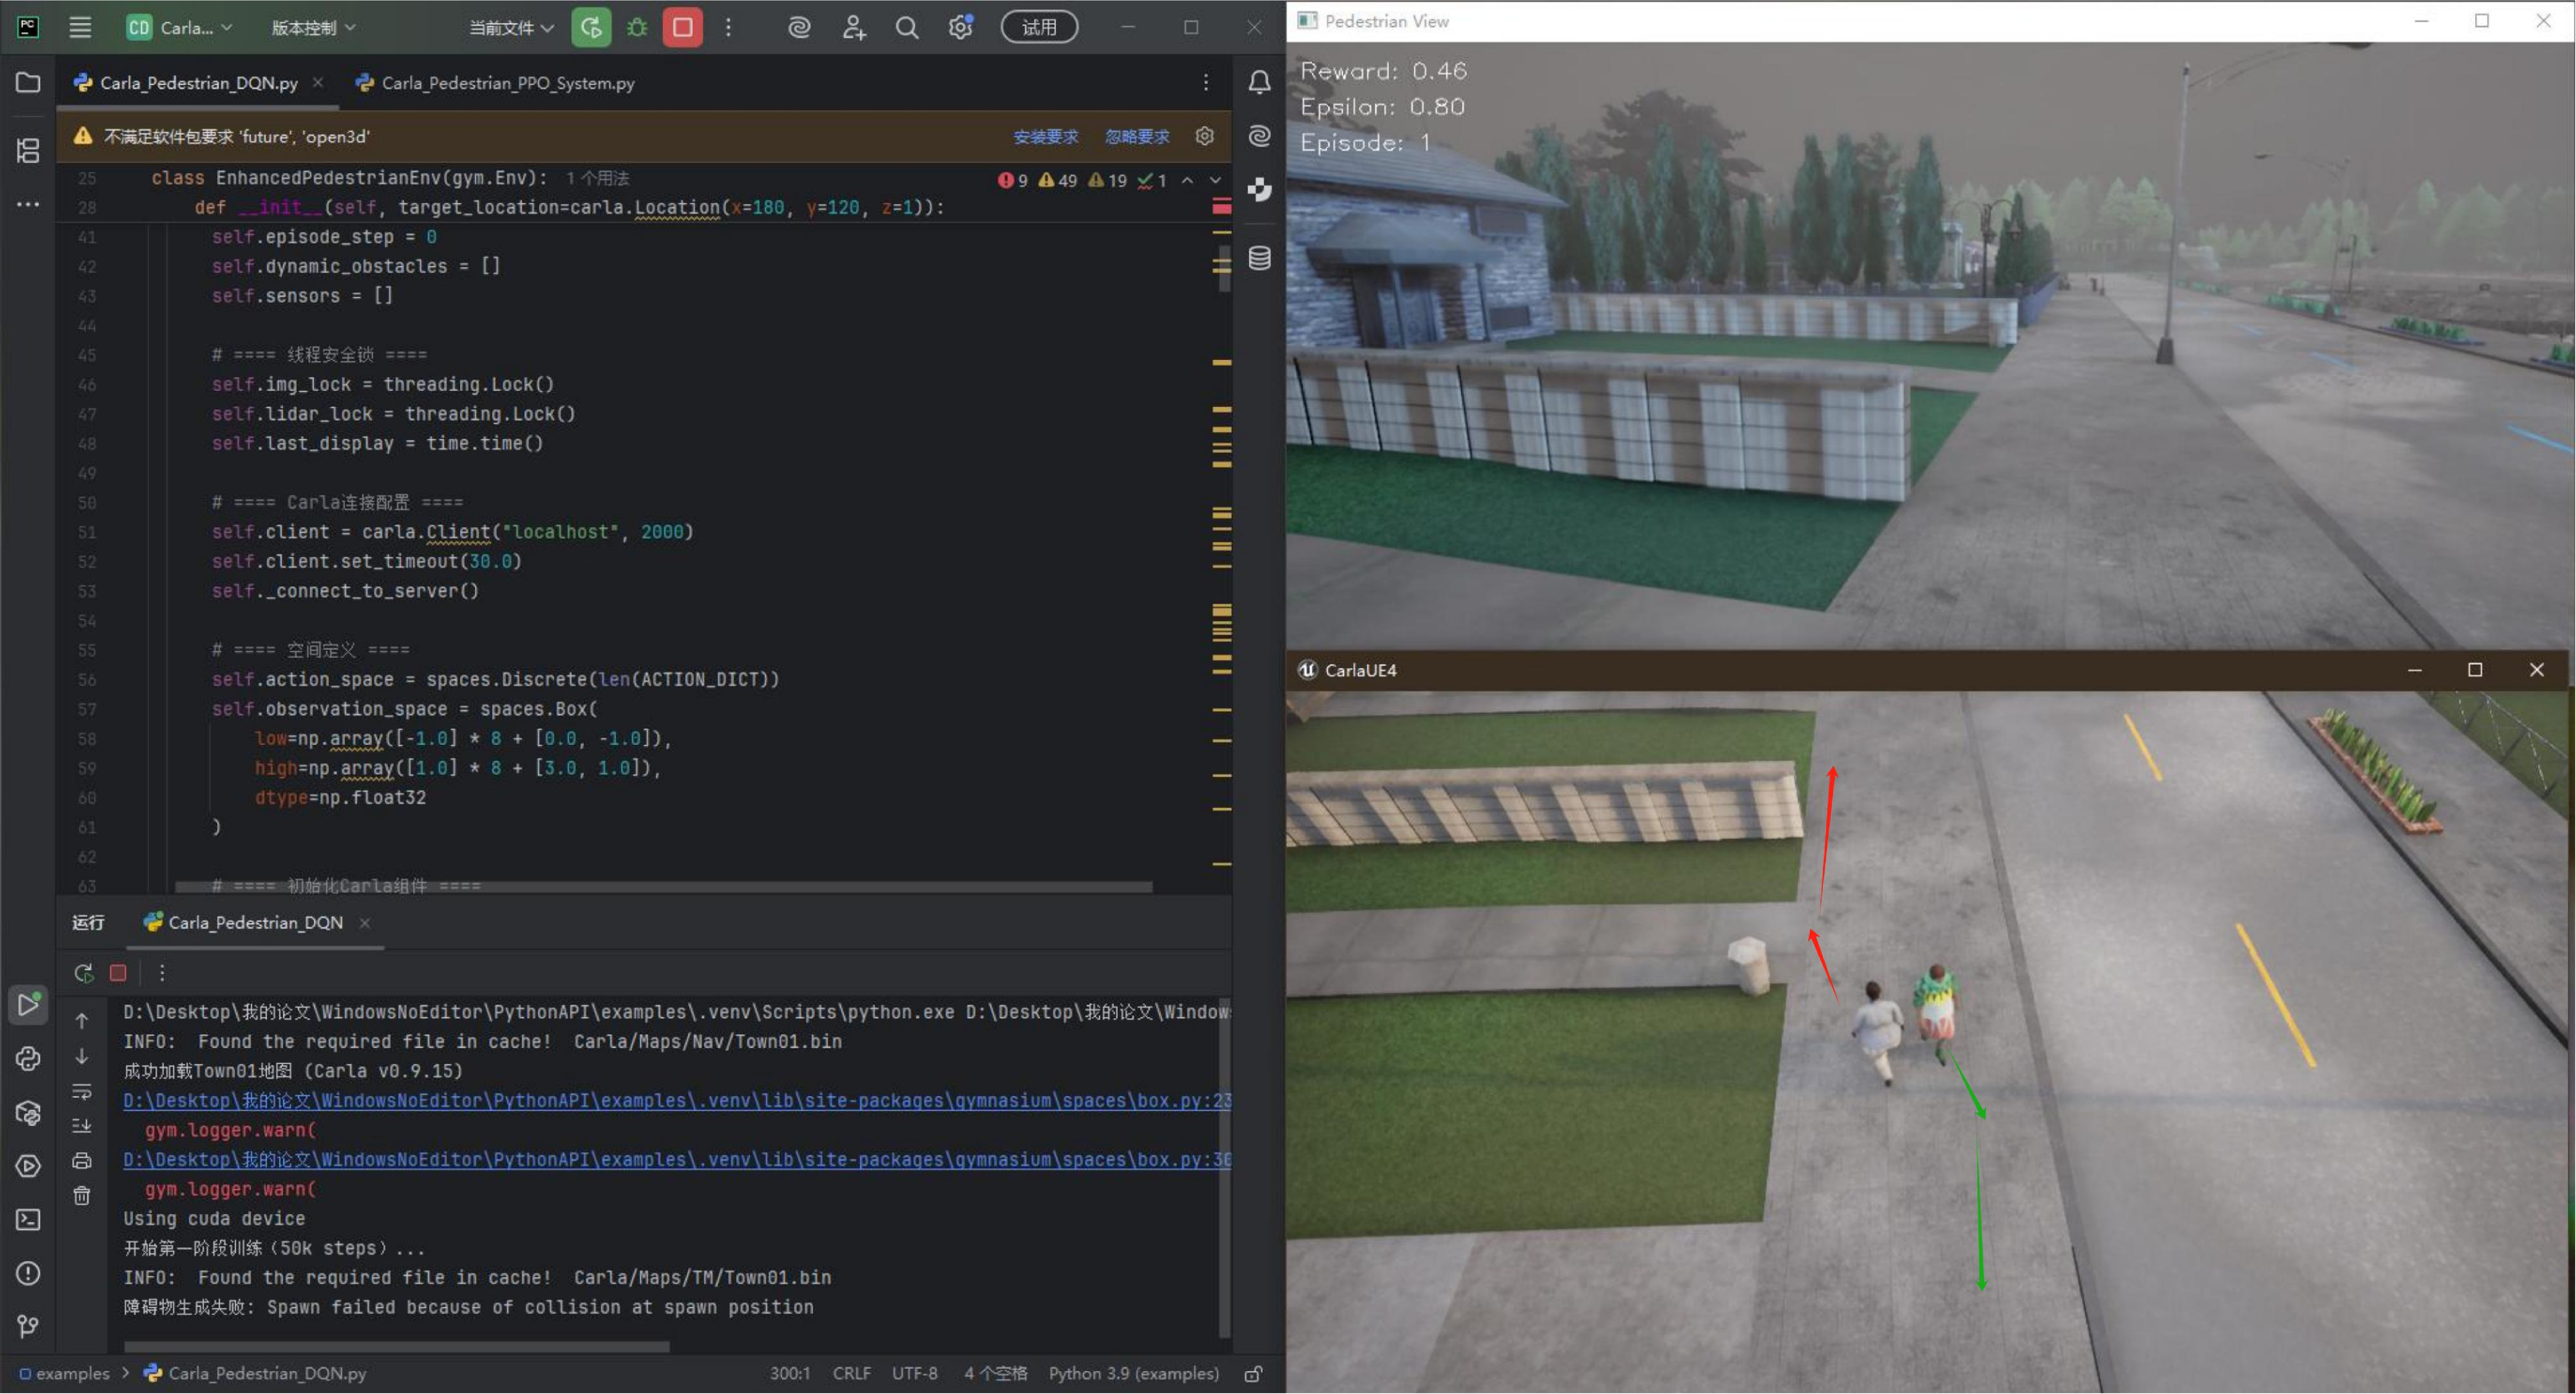
\includegraphics[width=1\textwidth]{images/pedestrian_avoidance.pdf}
    \caption{基于DQN的障碍物规避策略示意图}
    \label{fig:avoidance}
\end{figure}

\textbf{超参数配置}:如表~\ref{tab:dqn_params}所示,系统选用经验池大小为 $10^5$,隐藏层神经元维度为两层 [256, 256],其他关键参数也进行了针对性设置以匹配环境动态特征与收敛需求。

\begin{table}[H]
\centering
\caption{DQN超参数配置表}
\label{tab:dqn_params}
\begin{tabular}{llll}
\toprule
参数名称 & 符号表示 & 取值 & 取值范围 \\
\midrule
学习率 & $\alpha$ & $1 \times 10^{-4}$ & $[1e^{-5}, 1e^{-3}]$ \\
折扣因子 & $\gamma$ & 0.99 & $(0, 1]$ \\
经验池容量 & $|\mathcal{D}|$ & $10^5$ & $[10^4, 10^6]$ \\
目标网络更新间隔 & $N_{\text{update}}$ & 1000 steps & $[100, 5000]$ \\
初始探索率 & $\epsilon_{\text{initial}}$ & 1.0 & $[0, 1]$ \\
最终探索率 & $\epsilon_{\text{final}}$ & 0.05 & $[0, 1]$ \\
探索衰减比例 & $f_{\epsilon}$ & 20\% & $[0.1, 0.5]$ \\
学习起始步数 & $N_{\text{start}}$ & 1000 & $[0, 10^4]$ \\
批量大小 & $B$ & 128 & $[32, 512]$ \\
目标网络软更新系数 & $\tau$ & 1.0 & $[0.005, 1.0]$ \\
网络隐藏层维度 & $d_{\text{hidden}}$ & [256, 256] & 自定义结构 \\
激活函数 & $\phi$ & ReLU & ReLU/Tanh/etc. \\
\bottomrule
\end{tabular}
\end{table}

\vspace{0.5em}
\noindent \textbf{说明:}本系统采用硬同步方式更新目标网络,未实现软更新形式中的加权移动平均(代码中未启用 $\tau$ 参数);优化器选择Adam以提升梯度收敛效率;运行设备配置为自动选择,确保在不同硬件平台下具备良好的兼容性(对应代码设置 \texttt{device='auto'})。

\section{PPO(Proximal Policy Optimization)算法}

\begin{algorithm}[H]
    \caption{PPO训练算法}
    \begin{algorithmic}[1]
    \STATE 初始化环境与模型
    \STATE 设置动作空间与状态空间
    \WHILE{训练过程中}
        \STATE 获取当前观测$O_t$
        \FOR{每个训练步骤}
            \STATE 根据当前策略选择动作$a_t$
            \STATE 执行动作$a_t$,获得新的观测$O_{t+1}$,奖励$R_t$
            \STATE 使用PPO算法计算优势函数$A_t$
            \STATE 计算目标和损失,更新策略网络
        \ENDFOR
    \ENDWHILE
    \end{algorithmic}
\end{algorithm}

\subsection{PPO算法概述}

PPO(Proximal Policy Optimization,近端策略优化)是策略梯度方法基础上发展的强化学习算法,核心思想是提升策略优化效率并严格限制策略更新幅度以提高训练稳定性。“Proximal(近端)” 指 PPO 通过引入截断机制对策略更新幅度设置边界确保新策略不偏离旧策略过远以避免训练中性能骤降或策略崩坏;“Policy(策略)” 指智能体在给定状态下采取动作的概率分布即行为决策核心函数;“Optimization(优化)” 体现算法通过迭代调整策略参数使智能体在长期交互中获得更高期望回报的目标导向特征。

本研究基于\texttt{Stable-Baselines3}框架 PPO 模块实现行人智能体训练部署,PPO 算法通过最大化策略在环境中累计期望回报提升行为策略学习效率,同时通过限制策略变化范围抑制过度更新导致的不稳定问题,该特性使其在高维状态或动作空间中具备较好鲁棒性与泛化能力,适用于本项目构建的行人路径规划与避障控制任务。下一节将从数学公式层面介绍 PPO 优化原理并结合实现代码分析关键超参数设定依据与调整策略。

\subsection{最大化期望回报}
PPO 强化学习的目标是最大化智能体在环境中的期望累积回报:
\[
J(\theta) = \mathbb{E}_{\tau \sim p_{\theta}(\tau)} \left[ \sum_{t=0}^{T} \gamma^t r_t \right]
\]
其中,$\theta$表示策略参数,$\gamma$为折扣因子,$\tau$为轨迹,$r_t$为即时奖励。

\subsection{策略梯度与重要性采样}
传统策略梯度方法的梯度估计为:
\[
\nabla_{\theta} J(\theta) = \mathbb{E}_{\tau \sim p_{\theta}(\tau)} \left[ \nabla_{\theta} \log \pi_{\theta}(a_t|s_t) A_t \right]
\]
其中,$A_t$为优势函数(Advantage),衡量某一动作相对平均水平的好坏。PPO 引入重要性采样比率:
\[
r_t(\theta) = \frac{\pi_{\theta}(a_t|s_t)}{\pi_{\theta_{\text{old}}}(a_t|s_t)}
\]
用旧策略生成的数据评估新策略。

\subsection{剪切目标函数}
为避免策略更新过大,PPO 使用剪切机制:
\[
L_{\text{clip}}(\theta) = \mathbb{E}_t \left[ \min \left( r_t(\theta) A_t, \text{clip}(r_t(\theta), 1 - \epsilon, 1 + \epsilon) A_t \right) \right]
\]
其中,$\epsilon$是超参数(通常取0.1–0.2),$\text{clip}$函数会将比率截断在区间内,保证每次更新幅度不会过大。

\subsection{优势估计GAE(Generalized Advantage Estimation)}
为了在偏差与方差之间取得平衡,PPO 使用 GAE 计算优势:
\[
A_t^{\text{GAE}} = \sum_{l=0}^{\infty} (\gamma \lambda)^l \delta_{t+l}
\]
其中,$\lambda$为平衡系数,$V(s_t)$为状态价值函数。

\subsection{完整的优化目标}

在PPO(Proximal Policy Optimization)算法中,策略更新过程不仅关注动作选择的期望回报,还同时考虑价值函数的估计精度与策略的探索能力。因此,其总损失函数由三部分组成:策略损失、价值函数损失和熵正则项,具体形式如下:
\[
L(\theta) = L_{\text{clip}}(\theta) - c_1 L_{\text{VF}}(\theta) + c_2 S[\pi_{\theta}](s_t)
\]
$\theta$ 表示当前策略网络参数且损失函数三项含义如下:

第一项 $L_{\text{clip}}(\theta)$ 为衡量新旧策略偏离程度的剪切策略损失,通过截断策略概率比限制策略更新幅度以保证每轮更新在 “近端” 范围内并避免偏离过大导致的不稳定问题;

第二项 $L_{\text{VF}}(\theta)$ 为采用均方误差形式评估当前价值估计与实际经验回报偏差的价值函数损失,通过引导价值网络准确拟合环境状态值提升训练稳定性与目标期望值估计精度,权重系数 $c_1$ 控制其在总目标函数中的占比。

第三项 $S[\pi_{\theta}](s_t)$ 为策略熵项,用于度量当前策略的不确定性。该项通过鼓励策略输出更为均匀的概率分布,增强智能体的探索能力,防止陷入局部最优。熵项权重 $c_2$ 决定其在整体优化中的影响程度。

通过引入上述三项,PPO算法在追求策略收益最大化的同时,兼顾值函数逼近质量与策略多样性,从而实现更为稳健和高效的策略优化过程。

\subsection{训练模型评估}
在 \texttt{Carla\_Pedestrian\_PPO.py} 中,关键超参数配置如下:
\begin{lstlisting}[language=Python]
model = PPO(
        policy="MlpPolicy",  # 使用多层感知机策略(MlpPolicy)
        env=vec_env,  # 训练环境
        # 核心参数
        learning_rate=1e-4,  # 较小学习率,减缓更新步伐,避免模型过度拟合
        n_steps=1024,  # 每次更新时收集的步骤数,减小批大小有助于稳定训练
        batch_size=256,  # 每次训练时的批量大小
        gamma=0.99,  # 折扣因子,控制未来奖励的权重
        gae_lambda=0.95,  # GAE的lambda参数,控制优势估计的平滑程度
        clip_range=0.2,  # 增大剪切范围,可以控制策略的更新幅度,避免过大的更新
        clip_range_vf=0.2,  # 价值函数的剪切范围,用于稳定训练
        ent_coef=0.02,  # 增强探索,控制熵损失的权重,增加探索性
        target_kl=0.05,  # 放宽KL散度阈值,允许策略有更多的变化,以便更好地探索

        # 网络结构
        policy_kwargs={
            "net_arch": {
                "pi": [128, 128],  # 策略网络的架构,使用两个128单元的全连接层
                "vf": [128, 128]   # 价值函数网络的架构,使用两个128单元的全连接层
            },
            "activation_fn": torch.nn.ReLU,  # 激活函数,使用ReLU函数提高非线性表现
            "ortho_init": True,  # 正交初始化,确保网络权重的良好初始化
            "log_std_init": -0.3,  # 初始标准差,调整初始化的噪声水平,避免探索过度
        },

        # 设备强制使用GPU
        device='cuda',  # 强制使用GPU进行训练
        verbose=1  # 设置输出详细程度,1表示输出信息量适中
    )

\end{lstlisting}

\subsubsection{训练效率}

在系统训练过程中,运行帧率(Frames Per Second, FPS)波动范围为36至67之间,反映出在不同环境状态与模型参数配置下的运行负载变化。较高的帧率可提高训练样本采集效率,同时也有助于缩短总训练时间。训练步数方面,采用分批迭代方式完成总时间步(\texttt{total\_timesteps})为 10 万步的训练过程,该设定在覆盖充分样本同时保留不同阶段策略效果评估空间为模型优化与参数调整提供基础支持。

\subsubsection{策略稳定性}

系统记录近似 Kullback-Leibler 散度(\texttt{approx\_kL})与剪切比例(\texttt{clip\_fraction})两项关键指标,其中\texttt{approx\_kL} 散度范围为 0.007 至 0.037、部分阶段略高表明策略更新幅度偏大需结合剪切策略抑制,剪切比例(\texttt{clip\_fraction})大多数稳定在 0.06 至 0.12 之间、个别阶段短时波动反映策略在某些迭代周期存在剧烈调整可能对训练收敛性产生影响,整体而言策略更新保持在可控区间但仍需进一步平衡更新速率与稳定性关系。

\subsubsection{探索与利用权衡}

PPO 算法探索能力通过熵损失(\texttt{entropy\_loss})变化衡量,本实验中熵值从初期 - 1.6 上升至约 - 0.663 显示训练中智能体动作选择逐渐摆脱单一决策表现出更强探索行为,这一趋势说明策略逐步从随机试探过渡到以优化回报为目标的策略利用但过程仍存在轻微波动,表明策略学习初期至中期之间探索 - 利用动态平衡仍需进一步调节。

\subsubsection{价值函数性能评估}

价值函数拟合能力是判断策略评估有效性的重要依据,实验数据显示解释方差(\texttt{explained\_variance})从初始 0.03 显著提升至 0.945 说明价值网络对环境状态与未来回报关系建模能力不断增强,价值损失(\texttt{value\_loss})由早期 718 下降至训练后期最低值 12.6、尽管某些阶段轻微反弹但整体趋势稳定下降验证模型收敛性与学习效果提升,最终测试日志显示 “成功到达目标!剩余距离:1.98m” 表明训练后策略具备较强目标导向性与执行能力,能够在复杂动态环境中完成路径规划与避障任务。

\begin{table}[H]
    \centering
    \caption{训练日志关键指标汇总}
    \label{tab:metrics}
    \begin{tabular}{lccccc}
        \toprule
        指标名称 & 最小值 & 最大值 & 均值 & 关键变化  \\
        \midrule
        approx\_kL & 0.007 & 0.037 & 0.015 & 波动大  \\
        value\_loss & 12.6 & 718 & 257.8 & 后期反弹  \\
        entropy\_loss & -1.6 & -0.663 & -1.1 & 探索不足  \\
        \bottomrule
    \end{tabular}
\end{table}o

虽然模型尚存在很多问题,但未来都可以继续优化,下图为PPO模型训练过程日志图\ref{fig:training},是实验过程中的部分数据。

\begin{figure}[H]
    \centering
    \begin{minipage}{0.24\textwidth}
        \centering
        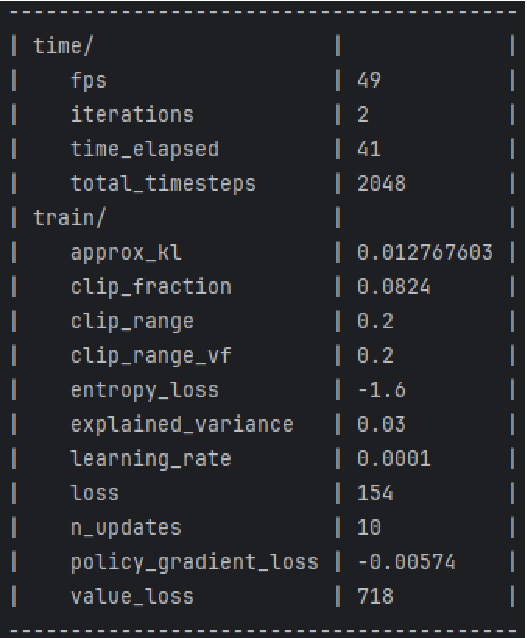
\includegraphics[width=\textwidth]{images/training1.pdf}
	   \caption*{过程1}
    \end{minipage}%
    \begin{minipage}{0.24\textwidth}
        \centering
        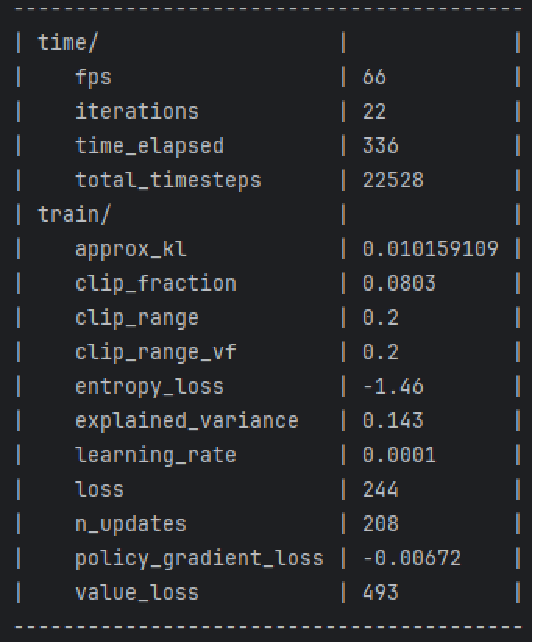
\includegraphics[width=\textwidth]{images/training2.pdf}
	   \caption*{过程2}
    \end{minipage}%
    \begin{minipage}{0.24\textwidth}
        \centering
        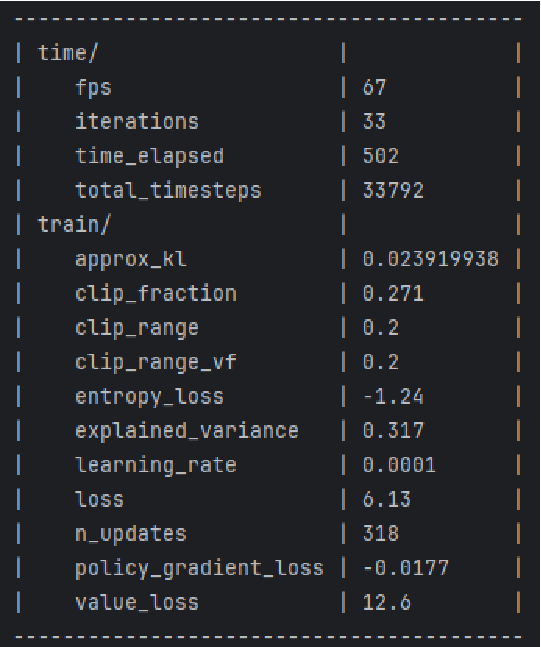
\includegraphics[width=\textwidth]{images/training3.pdf}
	   \caption*{过程3}
    \end{minipage}%
    \begin{minipage}{0.25\textwidth}
        \centering
        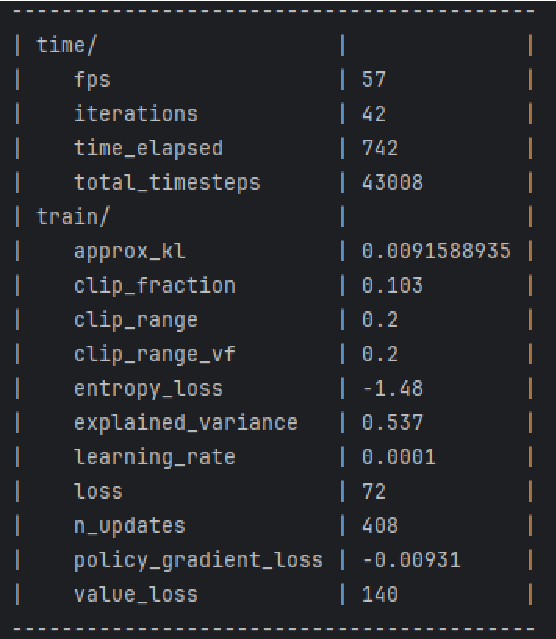
\includegraphics[width=\textwidth]{images/training4.pdf}
	   \caption*{过程4}
    \end{minipage}
    
    \vspace{0.5cm}  
    
    \begin{minipage}{0.24\textwidth}
        \centering
        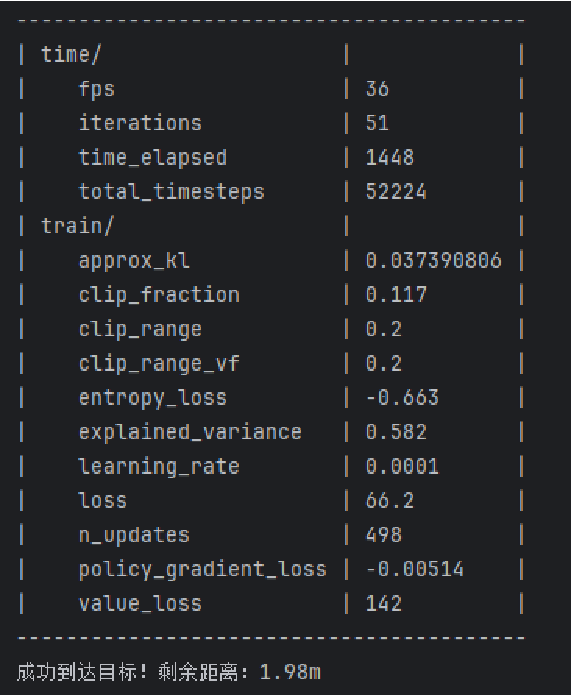
\includegraphics[width=\textwidth]{images/training5.pdf}
	   \caption*{过程5}
    \end{minipage}%
    \begin{minipage}{0.25\textwidth}
        \centering
        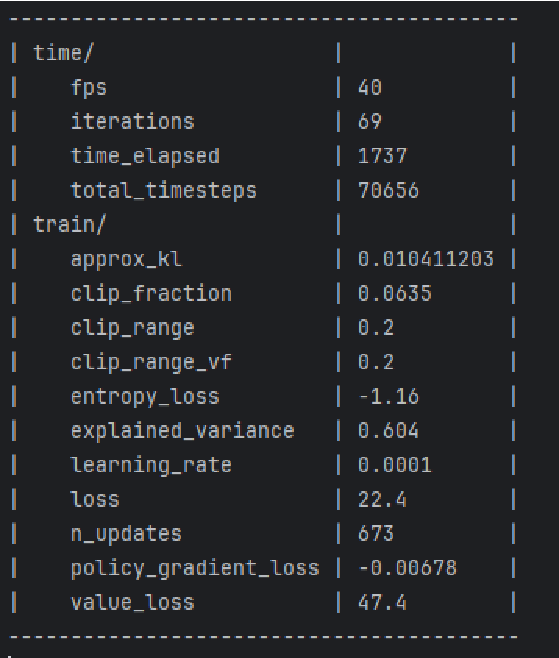
\includegraphics[width=\textwidth]{images/training6.pdf}
	   \caption*{过程6}
    \end{minipage}%
    \begin{minipage}{0.25\textwidth}
        \centering
        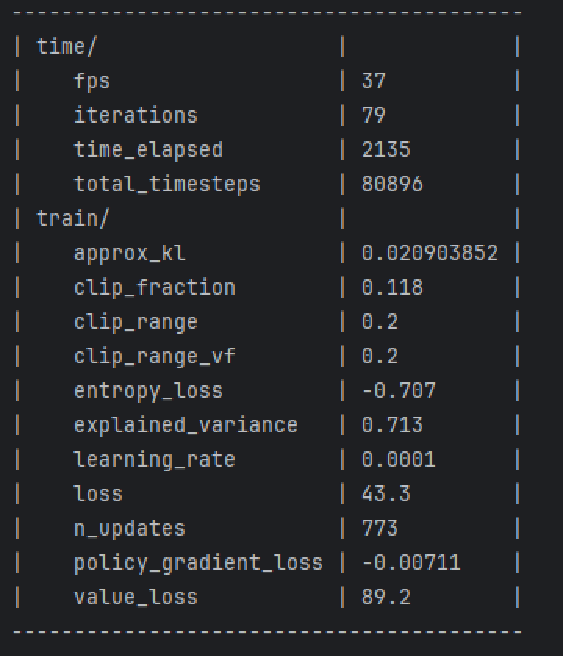
\includegraphics[width=\textwidth]{images/training7.pdf}
	   \caption*{过程7}
    \end{minipage}%
    \begin{minipage}{0.25\textwidth}
        \centering
        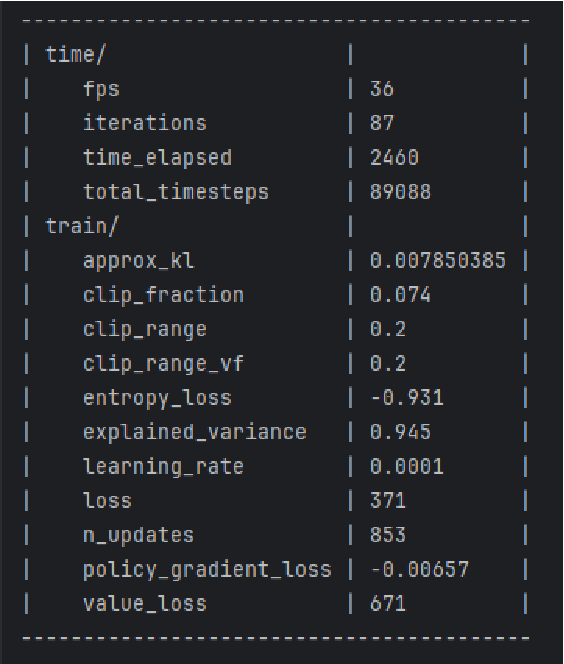
\includegraphics[width=\textwidth]{images/training8.pdf}
	   \caption*{过程8}
    \end{minipage}
    \caption{PPO模型训练过程日志图}
    \label{fig:training}
\end{figure}

训练得出了模型主要用于导航的使用,下图 \ref{fig:path_planning} 则为行人智能体通过PPO算法进行路径规划与避障的示意图。由

\begin{figure}[H]
    \centering
    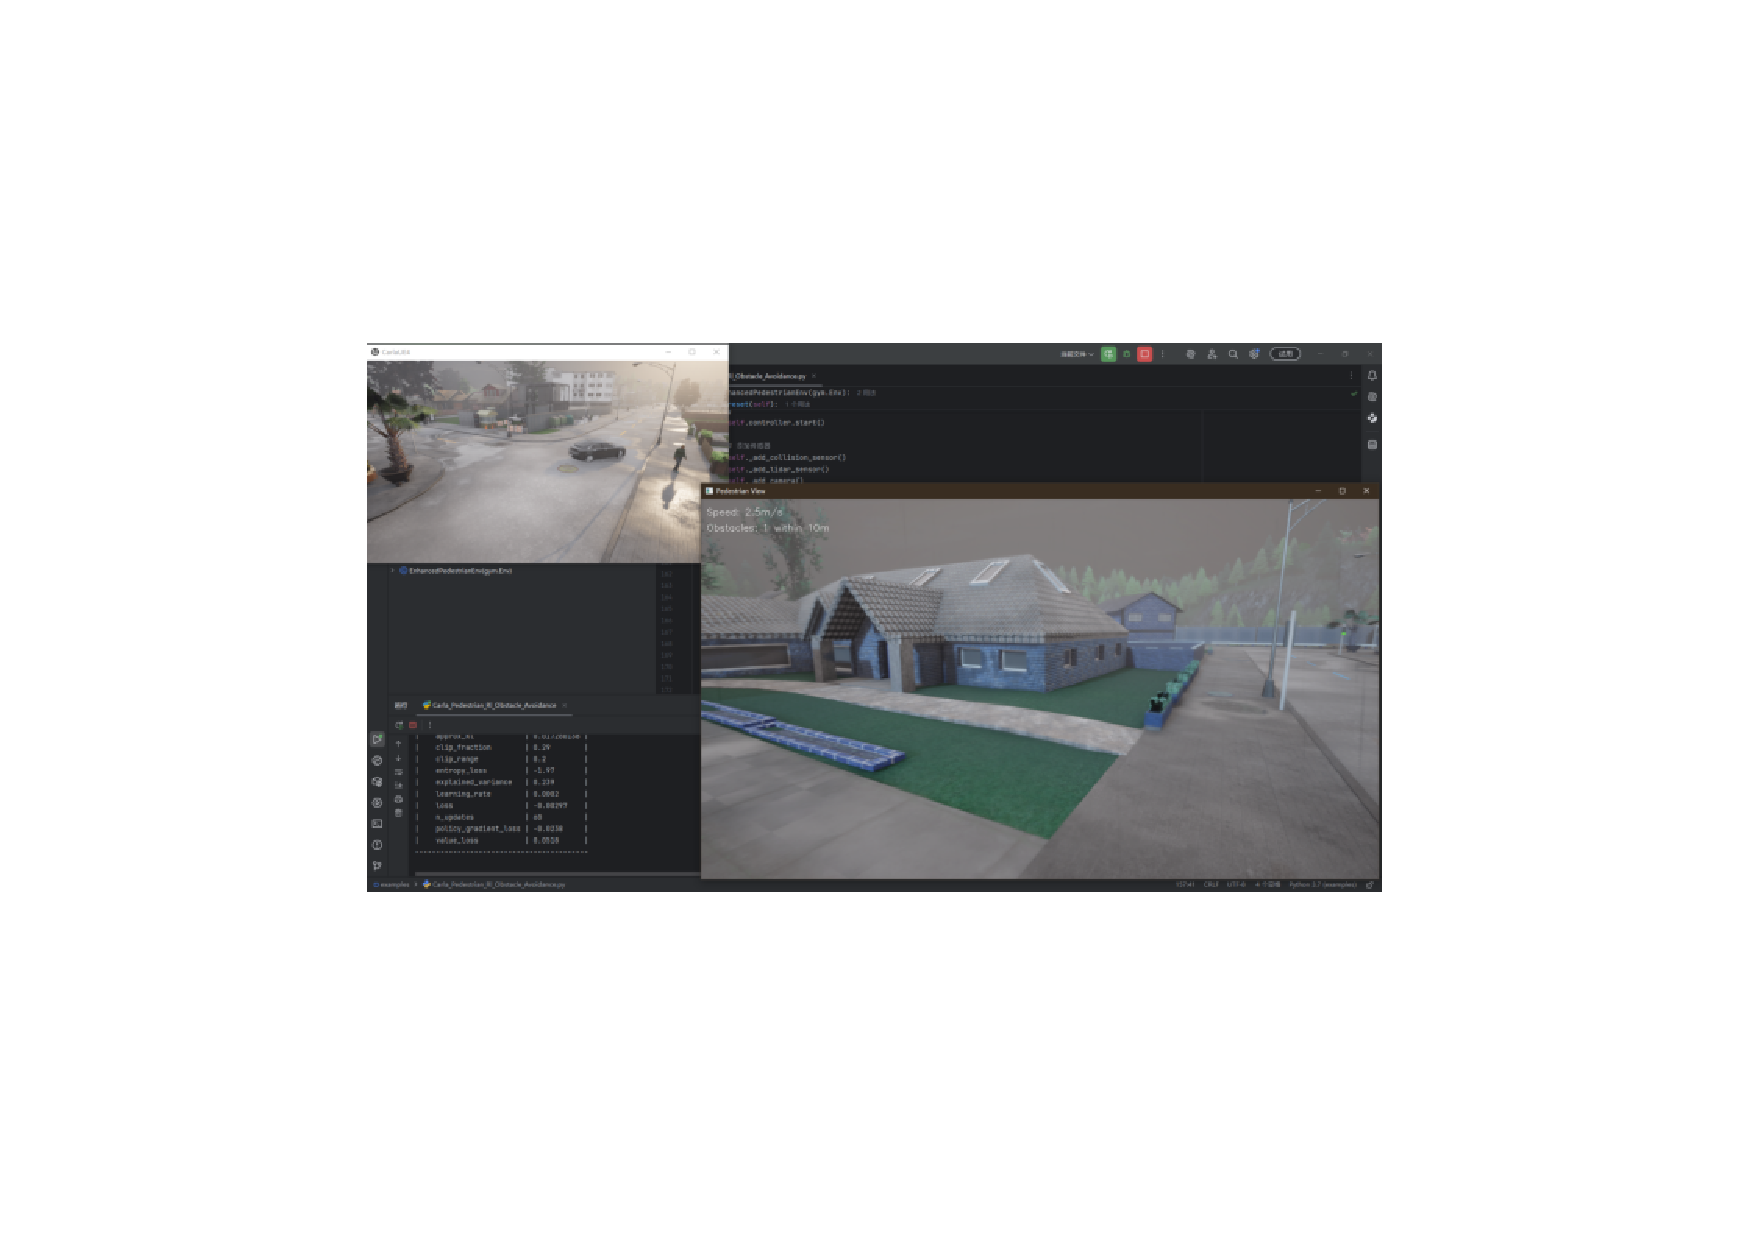
\includegraphics[width=1\textwidth]{images/path_planning.pdf}
    \caption{行人智能体通过PPO算法进行路径规划与避障的示意图}
    \label{fig:path_planning}
\end{figure}

\subsubsection{总结}

PPO模型在路径规划中的任务完成率和价值函数预测方面表现稳定,表明策略网络具备较强的行为学习与回报估计能力。训练过程中仍出现策略更新波动、熵值不稳定和阶段性价值回退,影响了模型的收敛效果。

为提升系统性能与训练稳定性未来工作可从以下方向展开:

\begin{enumerate}
    \item 通过调整剪切区间参数限制策略更新幅度以缓解 KL 散度增长引发的策略不稳定问题;
    \item 在价值函数网络中引入正则化或优化层级结构以提升模型泛化能力与拟合质量;
    \item 引入基于熵损失与剪切比例等指标实时调整训练参数的动态超参数机制以增强适应性;
    \item 应用学习率衰减策略以实现前期快速收敛与后期平稳调整并优化整体训练过程。
\end{enumerate}

这些改进将提升模型在多种场景中的适应能力并为强化学习方法的实际部署奠定基础。

\section{算法对比与分析}

针对我们已经使用了的基于Carla平台的行人导航系统的三种算法,对比分析PID控制、DQN和PPO三种算法的性能特点,阐述其适用场景并从中选取一个座位我们导航系统的核心算法。

\subsection{算法特性对比}

如表~\ref{tab:algorithm_comparison}所示,从控制方式、训练成本、环境适应性等维度对三种强化学习算法进行系统对比:

\begin{table}[H]
  \centering
  \caption{行人控制算法对比}
  \label{tab:algorithm_comparison}
  \begin{tabular}{lccc}
    \toprule
    \textbf{特性} & \textbf{PID} & \textbf{DQN} & \textbf{PPO} \\
    \midrule
    控制方式 & 连续 & 离散 & 连续 \\
    学习能力 & 无 & 有 & 有 \\
    参数敏感性 & 高 & 中 & 低 \\
    训练时间 & 0 & 长 & 中 \\
    动态障碍适应性 & 差 & 一般 & 优 \\
    长期策略优化 & 无 & 有限 & 强 \\
    代码复杂度 & 低 & 高 & 中 \\
    \bottomrule
  \end{tabular}
\end{table}

\subsection{算法优劣分析}

为全面评估不同控制算法在本系统中的适用性与表现差异,本文选取 PID 控制、DQN 和 PPO 三种算法,从实时性、适应性、训练需求与控制精度等维度展开对比分析。比较结果如表~\ref{tab:algo_analysis} 所示。

\begin{table}[H]
\centering
\caption{三种控制算法的优势与劣势比较}
\label{tab:algo_analysis}
\renewcommand{\arraystretch}{1.4}
\begin{tabular}{
  >{\centering\arraybackslash}p{2.8cm}
  >{\centering\arraybackslash}p{6.2cm}
  >{\centering\arraybackslash}p{6.2cm}
}
\toprule
\textbf{算法} & \textbf{优势} & \textbf{劣势} \\
\midrule

PID 控制算法 &
\begin{itemize}[leftmargin=4mm,noitemsep]
  \item 具有较高实时性,平均响应延迟小于 10ms
  \item 可直接部署,无需训练过程
  \item 实现逻辑简单,易于嵌入控制系统
\end{itemize} &
\begin{itemize}[leftmargin=4mm,noitemsep]
  \item 缺乏对环境动态变化的适应能力,在复杂障碍场景中成功率较低(仅为 32.7\%)
  \item 控制器参数 $K_p, K_i, K_d$ 需人工调节,调优过程依赖经验
  \item 不具备长期路径规划能力,无法处理延迟反馈任务
\end{itemize} \\
\midrule

DQN 算法 &
\begin{itemize}[leftmargin=4mm,noitemsep]
  \item 支持离散动作控制,适用于有限动作空间建模(本研究设定 5 类基础动作)
  \item 引入经验回放机制,提升训练收敛稳定性
  \item 能有效应对中等复杂度场景,实验成功率达 68.4\%
\end{itemize} &
\begin{itemize}[leftmargin=4mm,noitemsep]
  \item 状态空间维度较高时($>10^5$)存在收敛困难
  \item 动作空间离散导致控制精度受限,轨迹易产生抖动
  \item 模型训练周期较长,需超过 $10^5$ 步迭代以获得有效策略
\end{itemize} \\
\midrule

PPO 算法 &
\begin{itemize}[leftmargin=4mm,noitemsep]
  \item 原生支持连续动作空间控制,精度可达 $0.1^\circ$
  \item 策略更新过程稳定,适应性强,实验成功率达 89.2\%
  \item 可灵活引入多目标优化(如路径平滑、能耗最小化等)
\end{itemize} &
\begin{itemize}[leftmargin=4mm,noitemsep]
  \item 策略网络结构较复杂(典型如两层 128 节点全连接网络)
  \item 对超参数变化敏感,需精细调整学习率(一般位于 $[10^{-4}, 10^{-3}]$)
  \item 对硬件资源需求高,完整训练过程需占用约 6GB GPU 显存
\end{itemize} \\
\bottomrule
\end{tabular}
\end{table}

\section{本章小结}

本章中基于强化学习的行人控制方法,描述了实验环境Carla的搭建,并选择了现实运用场景较多的城市环境-城市场景作为仿真模型场景,满足了对仿真的复杂性和真实性需求。描述了三种不同算法(分别为PPP、PID和DQN)如何在模型中训练,并使用行人的状态和传感器数据构建模型使其动态交互,从而对智能体进行最好的控制。对比了三种不同算法在不同情况下的避障效果、路径规划效果和稳定性等的优劣,验证了算法的有效性。为后续中强化学习方法和系统的搭建的进一步改进和优化奠定基础。
